% ============================================================
% BioDecisionBench — LaTeX includes for all generated figures
% (regenerate with: python3 gen_fig1_hero.py gen_fig2_transfer.py
%  gen_fig3_dynamics.py gen_fig4_ablation.py gen_tables.py)
% Tables: % Table 1: benchmark composition (generated by gen_tables.py)
\begin{table}[t]
\centering
\caption{BioDecisionBench composition. Rows are the 10 source families (canonical
task-id prefix map used by the training scheduler; \texttt{lg\_}/\texttt{protein\_homology} share the
\texttt{local\_snapshots} family). Task counts are per evaluation unit; ProteinGym's 217 assays
share one question type. Admission: 0 train/test sequence leaks after isolation;
1{,}984 conflicting-label groups quarantined (not majority-voted);
925{,}985 cross-task duplicate sequences kept isolated per task.}
\label{tab:benchmark}
\small
\begin{tabular}{lrrrrrrrrr}
\toprule
Family & Mod. & choice & noul & score & multi & Tasks & Train & Dev & Test
\\ \midrule
ProteinGym & P & -- & -- & 217 & -- & 217 & 415,201 & 140,300 & 140,810 \\
GUE & D & 28 & -- & -- & -- & 28 & 731,069 & 82,350 & 82,125 \\
RNAcompete & R & -- & -- & 14 & -- & 14 & 275,449 & 33,610 & 33,476 \\
GenomicBenchmarks & D & 1 & 7 & -- & -- & 8 & 516,071 & 57,251 & 162,541 \\
gene\_lan & D+P & -- & 8 & -- & -- & 8 & 104,130 & 12,897 & 12,973 \\
local\_snapshots & D+P & 5 & 2 & -- & -- & 7 & 69,469 & 6,894 & 7,048 \\
dnagpt\_pools & D & 3 & -- & -- & -- & 3 & 111,269 & 12,527 & 13,892 \\
TAPE & P & -- & -- & 2 & -- & 2 & 74,955 & 7,874 & 40,042 \\
DeepSTARR & D & -- & -- & 2 & -- & 2 & 804,576 & 81,140 & 82,372 \\
DeepLoc & P & -- & -- & -- & 1 & 1 & 16,878 & 5,462 & 5,963 \\
\midrule
\textbf{Total} & D42+P226+R14+8D & 37 & 17 & 235 & 1 & 290 & 3,119,067 & 440,305 & 581,242 \\
\bottomrule
\end{tabular}
\end{table}
 etc.
% ============================================================

% === Fig 1: hero — benchmark panorama + seed-averaged three-way ===
\begin{figure*}[t]
\centering
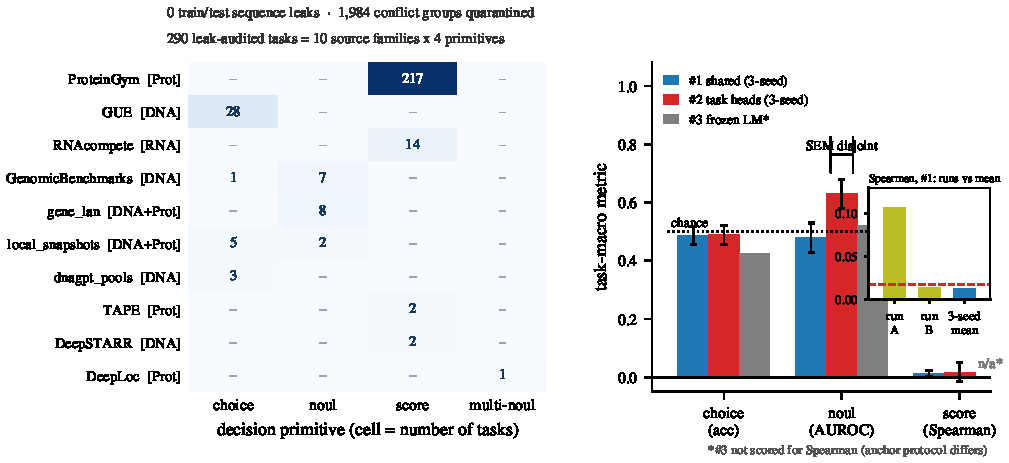
\includegraphics[width=0.98\textwidth]{figures/fig1_hero.pdf}
\caption{\textbf{BioDecisionBench and its headline comparison.}
\emph{Left:} 290 leak-audited tasks over 10 source families and 4 decision
primitives; the admission protocol leaves zero within-task train/test sequence
overlap (1{,}984 conflicting-label groups quarantined rather than majority-voted).
\emph{Right:} seed-averaged (3 seeds), matched-compute comparison per primitive
(mean$\pm$SEM over tasks). Per-task heads (\#2) beat the shared typed-decision
scorer (\#1) on noul (disjoint SEMs) and tie on choice/score; both trained arms
exceed the frozen candidate-likelihood baseline (\#3, not compute-matched).
\emph{Inset:} the methodological warning --- two single runs of the same
configuration give score Spearman 0.107 vs 0.015 for \#1; the 3-seed mean is 0.013.}
\label{fig:hero}
\end{figure*}

% === Fig 2: three operational checks on #1's claimed value ===
\begin{figure*}[t]
\centering
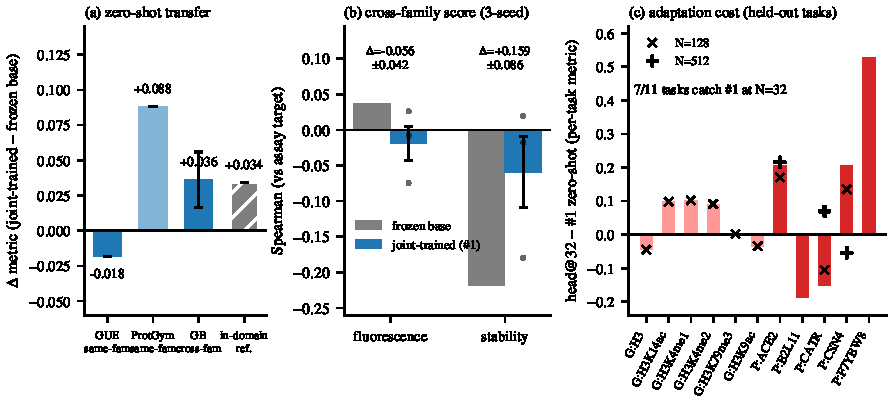
\includegraphics[width=0.98\textwidth]{figures/fig2_transfer.pdf}
\caption{\textbf{Three operational tests of the shared scorer's claimed advantages.}
(a) Zero-shot transfer to same-family held-out tasks is a wash (GUE $-0.018$,
ProtGym $+0.088$); cross-family transfer on GenomicBenchmarks is weakly positive
($+0.036$, SEM over 3 seeds), comparable to the in-domain reference ($+0.034$;
full2 configuration, not strictly matched).
(b) Cross-family \emph{score} transfer (TAPE, 3 seeds) does not hold: fluorescence
degrades ($\Delta=-0.056\pm0.042$); stability's apparent gain
($+0.159\pm0.086$) is regression of a pathological frozen baseline ($-0.218$)
toward zero --- trained absolute Spearman stays negative ($-0.059$).
(c) Adaptation cost: a fresh \#2 linear head catches \#1's zero-shot on 7/11
held-out tasks with only $N{=}32$ labels ($\times$: $N{=}128$, $+$: $N{=}512$).}
\label{fig:transfer}
\end{figure*}

% === Fig 3: training dynamics ===
\begin{figure*}[t]
\centering
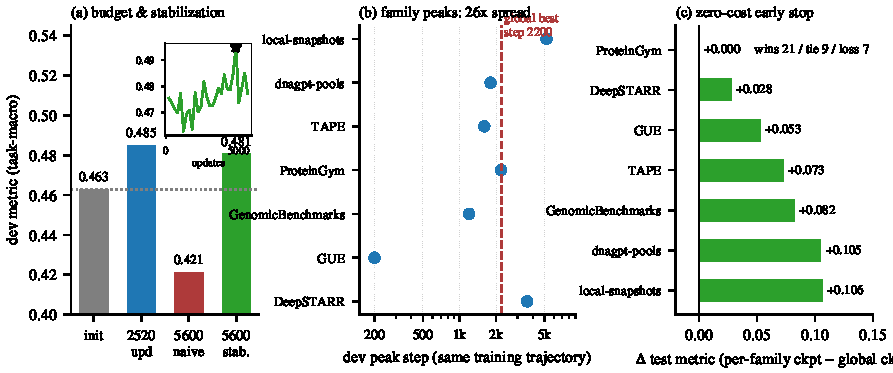
\includegraphics[width=0.98\textwidth]{figures/fig3_dynamics.pdf}
\caption{\textbf{Training dynamics under joint multi-task fitting.}
(a) Naive budget scaling destabilizes: 5{,}600 updates score \emph{below} init
(0.421) while 2{,}520 reaches 0.485; stabilization (warmup 0.15, grad clip 0.5,
dev early stop) recovers 0.481 at 5{,}600 --- a plateau, not overfitting
(inset: stabilized dev curve; star = selected checkpoint).
(b) Family-optimal dev peaks on the \emph{same} trajectory span steps 200--5{,}200
(26$\times$), while the global best sits at 2{,}200.
(c) Per-family early stopping (zero inference-time cost) dominates at family level
(all $\Delta\ge0$, mean $+0.063$); per task: 21 win / 9 tie / 7 loss vs the global
checkpoint.}
\label{fig:dynamics}
\end{figure*}

% === Fig 4: controlled mechanism ablations (panel b may move to appendix) ===
\begin{figure*}[t]
\centering
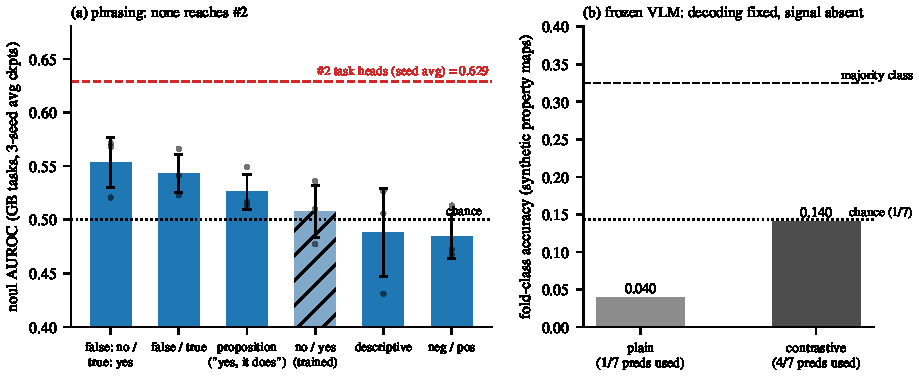
\includegraphics[width=0.98\textwidth]{figures/fig4_ablation.pdf}
\caption{\textbf{Controlled mechanism ablations.}
(a) Noul candidate phrasing on three seed-averaged stable checkpoints (same
weights; only candidate text varies). No phrasing reaches the per-task-head
reference (0.629, dashed); the best (``false: no / true: yes'', $0.553\pm0.023$)
beats the \emph{trained} phrasing (hatched) on all three seeds --- reversing the
single-checkpoint finding, i.e., inference-level ablations are also
checkpoint-dependent.
(b) Frozen VLM on synthetic property maps (multimodal route-A pilot): plain
candidate likelihood collapses to one class (acc 0.040, 1/7 classes used);
contrastive decoding removes the collapse (0.140, 4/7) but remains at chance ---
decoding fixed, signal absent.}
\label{fig:ablation}
\end{figure*}
